\chapter{IAM-A: copy error on single molecules}\label{ch:iama}

\section{What a molecule shows that an array cannot}

An array reports, at each site, the fraction of copies that are methylated. A sequencing read reports one molecule: a run of
CpGs, each methylated or not, on one strand of one cell's DNA. On a molecule that is otherwise methylated, an unmethylated CpG
between two methylated neighbors is a site the maintenance machinery failed to copy at the last division. That is the
\emph{copy error}, and it is the most direct reading of the writing process the book's physics is about.

\section{The statistic}

A molecule qualifies when it carries at least six CpG calls and at least 80~\% of them are methylated. Each interior call is
an opportunity; an unmethylated interior call with both neighbors methylated is an isolated error. The copy error is
\begin{equation}
  \varepsilon=\frac{\sum\text{isolated errors}}{\sum\text{opportunities}},
  \qquad E_{\rm hold}=\kB T\ln\frac{1-\varepsilon}{\varepsilon},
  \label{eq:eps}
\end{equation}
computed on the methylated channel only. The unmethylated channel is not used: there, bisulfite conversion failure dominates
the isolated calls. The chain requires at least 100,000 opportunities and reports the reading separately on odd and even
molecules as a repeat check. \derived{} for the form; the selection rules are \calibrated.

\section{The floor, the healthy reference and the ceiling}

If the cell holds each site with an energy $E$ against thermal kicks, a two-state Boltzmann factor gives the error that energy allows,
$\varepsilon=1/(1+e^{E/\kB T})$. \derived{} Three energies mark the gauge:
\begin{equation}
  \varepsilon_{\min}=\frac{1}{1+e^{M}},\qquad \varepsilon_0=\frac{1}{1+e^{\phi M}},\qquad \Hmin=H(\varepsilon_{\min}),\qquad \Href=H(\varepsilon_0).
  \label{eq:eps0}
\end{equation}
\begin{center}\small
\begin{tabular}{@{}llllll@{}}\toprule
mark & where & energy holding each site & thermal kicks win & entropy per site & set by \\\midrule
floor $\Hmin$ & left & one full ATP, $M=20.94\,\kB T$ & 1 in $1.24\times10^{9}$ & $2.5\times10^{-8}$ bits & $M$ alone \calc \\
healthy reference $\Href$ & middle & $3.41\,\kB T$ & 1 in 31 ($\varepsilon_0=0.032$) & $0.2043$ bits & healthy cells \measured \\
ceiling & right & none & every other time ($\varepsilon=\tfrac12$) & 1 bit & physics \derived \\\bottomrule
\end{tabular}\end{center}
The floor is where thermal kicks win against everything one ATP can buy, and no cell comes near it. The healthy reference is where healthy
cells actually hold their sites: the holding energy measured across 56 healthy cell types, $3.41\,\kB T$ (public single-molecule files, rebuilt from them by one committed
script), gives $\phi=0.1628$ of one ATP
(Chapter~\ref{ch:landauer}), $\varepsilon_0=0.032$ and $\Href=0.2043$ bits. Healthy cell types spread around it (copy error 0.024--0.042),
so about half hold their sites better than $\Href$; none approaches $\Hmin$. The distance between floor and reference is the cell's
efficiency, $\phi$. Thermodynamics bounds the holding energy by the free energy spent per renewal (one ATP sets the floor); the height
the cell actually holds is set by the kinetics of maintenance, the balance of restore and loss, $E_{\rm hold}=\kB T\ln(g/f)$
(Chapter~\ref{ch:landauer}). Restore and loss rates measured in the same cells return this balance by construction, since at steady state $g/f=(1-\varepsilon)/\varepsilon$;
deriving $\phi$ needs the writer's discrimination measured outside the cell, and is the central open problem of the cellular rung
(Chapter~\ref{ch:open}). \openprob

\section{The healthy position, and the reading}

Each healthy cell type sits at its own position $P$ relative to the healthy reference, measured once per cell type and per
read pipeline, and frozen:
\begin{equation}
  \text{IAM-A}=\frac{H(\varepsilon)}{P_{\rm cell}\,H(\varepsilon_0)},\qquad P_{\rm neutrophil}=1.149 .
  \label{eq:iama}
\end{equation}
\measured{} $P$ was measured on three healthy granulocyte donors (range 1.140--1.155, coefficient of variation 0.74~\%), on
whole read-level files of one public atlas~\cite{Loyfer2023}, with one named read-level pipeline. The average healthy cell type, $\Href$, then
sits at $A=1/P=0.870$ on the neutrophil's gauge, and the floor $\Hmin$ at $1\times10^{-7}$. \calc

\begin{center}\small
\begin{tabular}{@{}lll@{}}\toprule
test & result & \\\midrule
healthy donors on $\Href$ alone & 1.137--1.168 & \measured \\
healthy donors with $P$, leave-one-donor-out & 0.984--1.025 & \measured \\
odd/even molecule halves & differ by $\le0.002$ & \measured \\
2~\% of methylated calls removed: rise in $\varepsilon$ & $+0.0154$ to $+0.0155$ & \measured \\
the same rise read at each donor's held-out position & 1.273--1.313 & \calc \\
same cells on a second read pipeline, on $\Href$ alone & 0.70--0.79 & \measured \\\bottomrule
\end{tabular}
\end{center}
The last line is why $P$ is locked to a pipeline: the same cells read through a different alignment and extraction show a
different error. A new pipeline needs its own $P$, measured on healthy cells, before it can read anything.

Figure~\ref{fig:p4_donors} shows the three donors behind $P$, and Figure~\ref{fig:p4_iamacurve} shows where they sit on the curve that
IAM-A follows.

\begin{figure}[htbp]\centering
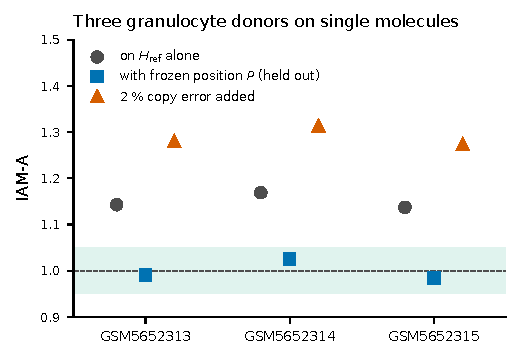
\includegraphics[width=0.62\textwidth]{figures/part6/fig_p4_08_donors.pdf}
\caption{The three healthy granulocyte donors on single molecules~\cite{Loyfer2023}. Circles: on the bare floor $\varepsilon_0$; squares: with the
frozen position $P$, each donor held out of its own $P$ (its odd and even molecule halves fall within the square); triangles: the same molecules
with 2~\% copy error added. The line is the floor $1/P$. \measured}
\label{fig:p4_donors}
\end{figure}
\begin{figure}[htbp]\centering
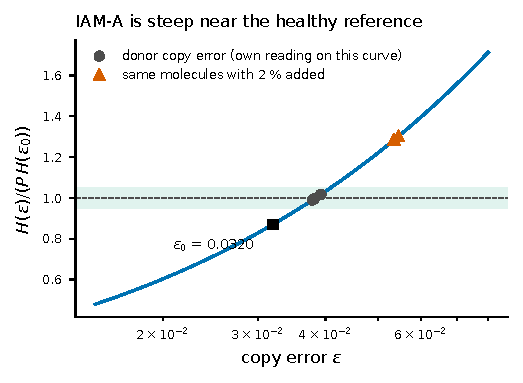
\includegraphics[width=0.6\textwidth]{figures/part6/fig_p4_08_curve.pdf}
\caption{$H(\varepsilon)/(P\,H(\varepsilon_0))$ against copy error, with $P=1.149$ and $\varepsilon_0=1/(1+e^{3.41})$. Square: the healthy reference $\Href$. Circles and
triangles: the donors' copy error and the same molecules with 2~\% added. A 2~\% rise moves the reading by about 0.3. \calc{} curve;
\measured{} points.}
\label{fig:p4_iamacurve}
\end{figure}

\begin{rulebox}
The floor and the reading must be defined by the same statistic on the same selection of molecules. A floor taken from a
different statistic (all-site copy error, with no filter on methylated molecules) misplaces healthy molecules several-fold.
\measured{} The chain enforces the rule.
\end{rulebox}

\section{One energy, many cells}

Read on the same 399 genomic windows for 153 samples of 56 healthy cell types, with no labels and no floor:
\begin{itemize}
\item the copy error ranges 0.024--0.042 and the holding energy $3.41\pm0.12\,\kB T$: close to one energy in every cell type;
\item on one physics floor (Eq.~\eqref{eq:eps0}) healthy cell types read 0.79--1.23, median 1.01; 27 of 56 inside Normal. One
      floor is not yet precise enough for an individual reading, which is why each cell type carries its own $P$;
\item on the 26,800 CpGs that all 56 cell types keep methylated, the same bits in every cell, the copy error still differs
      1.66-fold from the lowest (naive CD8 T cells, lung macrophages, B cells) to the highest (smooth muscle, heart
      fibroblasts, erythroid progenitors), and the difference is stable across donors (intraclass correlation 0.80);
\item cells do not sort by turnover: colon epithelium (a 3.4-day lifespan) and cardiomyocytes (56,000 days)~\cite{Sender2021} carry the same
      copy error, 0.031.
\end{itemize}
\measured{} for all four. The architecture of each cell's maintenance, not how often it is replaced, sets its position.

\section{Tumors}

The same statistic reads tumors against the same person's normal tissue with no reference group: in six early-onset
colorectal pairs the tumor's copy error is higher in all six, by 7--33~\%, and in oral squamous carcinoma in four of four, and in
three of the four when 5-hydroxymethylcytosine is removed (Chapter~\ref{part4:ch:reach}). \measured
